% This file was adapted from ICLR2022_conference.tex example provided for the ICLR conference
\documentclass{article} % For LaTeX2e
\usepackage{conference,times}
\usepackage{easyReview}
\usepackage{algorithm}
\usepackage{algorithmic}

% Optional math commands from https://github.com/goodfeli/dlbook_notation.
\input{math_commands.tex}

\usepackage{amsthm,amssymb}

\newtheorem{theorem}{Theorem}[section]
\newtheorem{corollary}{Corollary}[theorem]
\newtheorem{lemma}[theorem]{Lemma}
\newtheorem{definition}[theorem]{Definition}

% Please leave these options as they are
\usepackage{hyperref}
\hypersetup{
    colorlinks=true,
    linkcolor=red,
    filecolor=magenta,
    urlcolor=blue,
    citecolor=purple,
    pdftitle={Parity-Constrained Quantum Reservoir Computing for Image Classification: Formal Guarantees and Staged Simulation Evidence},
    pdfpagemode=FullScreen,
    }



\title{Parity-Constrained Quantum Reservoir Computing for Image Classification: \\ Formal Guarantees and Staged Simulation Evidence}

\author{Anonymous Authors \\
Anonymous Institution \\
\texttt{anonymous@anonymous.edu}}

\begin{document}


\maketitle

\begin{abstract}
Quantum reservoir computing has recently reported encouraging image-classification performance, yet many claims remain sensitive to fairness controls, measurement-policy confounds, and benchmark selection. We study a parity-constrained evaluation program for PCA-encoded image inputs and transverse-Ising-style reservoir dynamics, and we combine formal analysis with staged simulation evidence under fixed CPU-only constraints. First, we formulate advantage assessment as a bi-level optimization problem with matched preprocessing, readout family, observable budget, and search budget across quantum and classical branches, and we prove that parity-controlled deltas cannot exceed naive deltas computed with asymmetric policy optimization. Second, we formalize a non-monotone entanglement-utility criterion, showing that boundary derivative sign changes and interior concavity imply a unique interior optimum in coupling strength. Third, we derive an operator-attribution framework based on balanced crossed random effects and prove range and unbiasedness properties for operator-share estimators. Using a staged validation run over MNIST, Fashion-MNIST, EMNIST Balanced, Kuzushiji-MNIST, and a grayscale PCA variant of CIFAR-10, we observe conditional practical advantage on one hard dataset under a pre-registered acceptance tuple, consistent interior-optimum signatures in the tested regime, and strong operator-share estimates with parity-audit closure. These results support a guarded conclusion: formal guarantees are strong, empirical gains are conditional, and attribution quality improves materially when parity is enforced at the row level.
\end{abstract}

\section{Introduction}
Reservoir computing reduces training complexity by fixing nonlinear dynamics and learning only a linear or ridge readout, a perspective that has remained influential from echo-state and liquid-state systems to contemporary quantum reservoir variants \citep{jaeger2001,maass2002,lukosevicius2009}. In the quantum setting, this design is attractive because it avoids large variational parameter searches and can exploit hardware-native dynamics, while still supporting supervised prediction through classical post-processing. At the same time, recent quantum machine-learning literature repeatedly emphasizes that advantages depend on end-to-end assumptions, including data encoding, measurement design, and baseline parity \citep{biamonte2017,havlicek2019,schuld2020encoding,schuld2021kernel}. For image classification, these concerns are amplified when dimensionality reduction is applied upstream: if preprocessing already renders classes near-linearly separable, apparent gains can collapse under stronger controls.

This paper addresses a concrete open question: can PCA-encoded quantum reservoirs outperform strong classical reservoirs on image tasks once protocol parity is enforced, and what role does entanglement actually play in that outcome? Recent QELM and QRC studies report improved separability and accuracy in selected image and time-series settings \citep{delorenzis2024qelm,delorenzis2025entanglement,prieto2026superconducting,antoncich2026neutral,liu2026rydberg}. However, several papers also show that measurement policy optimization can shift performance substantially \citep{gross2026kernelop,aaraba2026quark,gross2026paulitransfer}, and multiple entanglement-focused studies indicate regime dependence with possible saturation \citep{delorenzis2025entanglement,askari2025spin,karimi2025kerr}. These observations motivate a methodology where advantage, mechanism, and attribution are evaluated in sequence rather than conflated.

Our study adopts that sequence explicitly. We first define a parity-constrained advantage objective with a pre-registered acceptance rule over a dataset ladder that includes MNIST and harder alternatives \citep{lecun1998mnist,xiao2017fashionmnist,cohen2017emnist,clanuwat2018kuzushiji,krizhevsky2009cifar}. We then isolate entanglement effects via controlled coupling-time ablations at fixed readout and observable settings, and we finally quantify operator-policy contribution using variance-component estimators under balanced design. This framing is deliberately hybrid: the paper is not purely theoretical and not purely benchmark-driven; instead, it develops formal guarantees and tests their operational implications in one integrated protocol.

The broader relevance extends beyond image classification. Fairness of comparator policies and identifiability of causal performance factors are recurring issues in reservoir and kernel methods, quantum and classical alike \citep{schuld2021kernel,gross2026kernelop,lukosevicius2009}. A parity-first methodology can therefore serve as a template for other domains where fixed-feature pipelines are evaluated under finite compute budgets, including molecular prediction and temporal forecasting \citep{beaulieu2024robust,ahmed2025chaotic,hamhoum2025mts,dibartolo2025multiphoton,kodali2025narma}.

\noindent\textbf{Contributions.} We make four contributions:
\begin{itemize}
\item We formalize practical-advantage testing as a parity-constrained bi-level program and prove a parity-shrink inequality showing that confound-controlled deltas are upper-bounded by naive asymmetric deltas.
\item We provide an interior-optimum theorem for entanglement-conditioned utility and show how boundary derivative signs and concavity yield a unique operating point under explicit assumptions.
\item We derive operator-share attribution estimators in a balanced crossed random-effects model, including range guarantees and unbiasedness identities used for interpretable causal decomposition.
\item We report staged simulation evidence with strict parity auditing and pre-registered acceptance constants, yielding conditional advantage on a hard benchmark, non-monotone mechanism support in the tested regime, and high operator-share estimates after rerun-level parity closure.
\end{itemize}

\section{Related Work and Motivation}
\subsection{Reservoir and Kernel Foundations}
Classical reservoir computing established an enduring abstraction: rich, fixed, high-dimensional dynamics followed by convex readout fitting \citep{jaeger2001,maass2002,lukosevicius2009}. Quantum supervised models can be interpreted through an analogous kernel lens, where data-encoding states define similarity geometry and measurement/readout specifies the final hypothesis class \citep{havlicek2019,schuld2021kernel}. This perspective clarifies two practical points that are central to our design. First, expressivity and generalization are heavily conditioned by encoding choices and induced spectra \citep{schuld2020encoding}. Second, training quality comparisons are meaningful only when readout classes and optimization budgets are controlled symmetrically across alternatives.

These points are not merely conceptual. In finite-sample settings, subtle differences in preprocessing and regularization grids can create large apparent improvements that do not survive parity checks. Classical RC literature already warns that tuning policy can dominate architecture conclusions \citep{lukosevicius2009}; recent QRC literature reinforces the same caution for quantum observables and kernelized readouts \citep{gross2026kernelop,aaraba2026quark}. Our protocol therefore treats parity not as a reporting footnote but as an explicit feasibility constraint in the optimization problem.

\subsection{Image-Centric QELM and QRC Evidence}
Image-focused quantum reservoir work has evolved rapidly. QELM studies combining PCA or learned compression with quantum dynamics and linear readouts have reported accuracy gains on MNIST-like and harder datasets, while often stressing computational efficiency from training only the readout layer \citep{delorenzis2024qelm,delorenzis2025entanglement}. Additional hardware and simulation studies suggest that scalable reservoir-style workflows can be competitive in selected classification tasks \citep{kornjaca2024largescale,prieto2026superconducting,antoncich2026neutral,liu2026rydberg,carles2025cqed,swierczewski2026optical,brusaschi2026inference,maier2025collider,assil2026memory}.

Yet the literature remains heterogeneous in benchmark hardness, noise assumptions, and comparator strength. MNIST remains a useful sanity floor but frequently saturates under modern pipelines, including classical baselines with simple feature engineering \citep{lecun1998mnist,xiao2017fashionmnist,cohen2017emnist}. For that reason, our study uses a ladder from MNIST to harder alternatives and explicitly conditions practical-advantage claims on hard-set performance. This design aligns with concerns in both QML surveys and recent QRC papers: isolated high scores on easy tasks do not establish robust advantage \citep{biamonte2017,delorenzis2025entanglement,gross2026paulitransfer}.

\subsection{Entanglement, Simulability, and Operator Confounds}
Recent studies increasingly agree that entanglement can improve embedding geometry in bounded regimes, but they also note saturation, regime dependence, and potential classical simulability of relevant dynamics \citep{delorenzis2025entanglement,askari2025spin,karimi2025kerr}. This is an important contrast to simplistic monotone narratives. If moderate coupling improves discrimination while strong coupling degrades utility, then mechanism claims should be framed through interior-optimum criteria, not endpoint comparisons.

A second recurring issue is operator-policy confounding. Kernel-based optimization of observables can materially change QRC performance \citep{gross2026kernelop,aaraba2026quark}, and related interpretability analyses show that measurement selection can control effective representation even when dynamics are fixed \citep{gross2026paulitransfer}. Without matched search budgets against classical feature-selection alternatives, architecture-level conclusions risk overstating quantum-dynamics effects. Our attribution model therefore decomposes variance contributions from operator policy and dynamics under balanced design, and reports shrinkage from naive to parity-controlled deltas as a first-class diagnostic.

\section{Problem Setting and Notation}
We consider supervised image classification after deterministic preprocessing. Let raw images be mapped to PCA features $\rvx \in \mathbb{R}^{d}$ through a shared operator $\Pi_d$. For each candidate configuration, a reservoir pipeline produces fixed features $\rvz(\rvx)$ followed by ridge readout. We compare quantum and classical branches under matched preprocessing, matched readout class, matched observable or feature dimension, and matched search budget.

\begin{definition}[Parity-Constrained Feasible Set]
Let $\vtheta_Q$ and $\vtheta_C$ denote quantum and classical policy parameters, respectively. The feasible set is
\begin{equation}
\Theta_{\mathrm{parity}} := \left\{(\vtheta_Q,\vtheta_C):\Pi_d^Q=\Pi_d^C,\ M_Q=M_C,\ \mathcal{R}_Q=\mathcal{R}_C,\ B_Q=B_C\right\},
\label{eq:theta_parity}
\end{equation}
where $M$ is observable/feature count, $\mathcal{R}$ is readout family and regularization grid, and $B$ is the search-budget accounting rule.
\end{definition}

For a dataset $d_s$, denote parity-controlled accuracy gap by $\Delta_{\mathrm{par}}^{(d_s)}$ and naive gap by $\Delta_{\mathrm{naive}}^{(d_s)}$. We use a pre-registered acceptance predicate
\begin{equation}
A_{\mathrm{adv}}^{(d_s)} = \mathbf{1}\!\left[\Delta_{\mathrm{par}}^{(d_s)} \ge \delta_{\min}\ \wedge\ p_{\mathrm{BH}}^{(d_s)} \le p_{\max}\ \wedge\ r^{(d_s)} \ge r_{\min}\right],
\label{eq:aadv}
\end{equation}
where $p_{\mathrm{BH}}$ is Benjamini-Hochberg corrected significance and $r$ is a robustness score across seeds.

The inner readout problem for either branch is ridge regression over fixed features:
\begin{equation}
\mathcal{L}(\mW) = \|\mW\mZ-\mY\|_F^2 + \lambda\|\mW\|_F^2,\qquad \lambda>0.
\label{eq:ridge_obj}
\end{equation}
Its closed-form optimum is
\begin{equation}
\mW^* = \mY\mZ^{\top}(\mZ\mZ^{\top}+\lambda\mI)^{-1}.
\label{eq:ridge_closed}
\end{equation}

The outer objective maximizes hard-set mean parity gap:
\begin{equation}
\vtheta^* \in \arg\max_{\vtheta\in\Theta_{\mathrm{parity}}}\ \frac{1}{|\mathcal{D}_{\mathrm{hard}}|}\sum_{d_s\in\mathcal{D}_{\mathrm{hard}}} \Delta_{\mathrm{par}}^{(d_s)}(\vtheta).
\label{eq:outer_obj}
\end{equation}
In this study the hard set is pre-registered as Fashion-MNIST, EMNIST Balanced, Kuzushiji-MNIST, and grayscale PCA CIFAR-10.

\subsection{Notation Summary}
Table~\ref{tab:notation} summarizes symbols that recur in the method and proofs.

\begin{table}[t]
\caption{Notation used in the formal development. The table groups optimization, mechanism, and attribution symbols that are referenced repeatedly in \secref{sec:method} and \secref{sec:results}. Symbols are defined in-line at first use and repeated here for readability during equation-heavy sections.}
\label{tab:notation}
\begin{center}
\small
\renewcommand{\arraystretch}{1.1}
\setlength{\tabcolsep}{4pt}
\begin{tabular}{ll}
\hline
Symbol & Meaning \\
\hline
$\rvx\in\mathbb{R}^{d}$ & PCA-compressed input vector \\
$\Pi_d$ & Shared preprocessing operator \\
$\mZ$ & Feature matrix from reservoir measurements \\
$\mW$ & Readout weight matrix \\
$\lambda$ & Ridge regularization parameter \\
$\Theta_{\mathrm{parity}}$ & Feasible set with matched protocol controls \\
$\Delta_{\mathrm{par}}$ & Parity-controlled quantum-classical gap \\
$\Delta_{\mathrm{naive}}$ & Naive gap under asymmetric policy optimization \\
$A_{\mathrm{adv}}$ & Practical-advantage acceptance predicate \\
$g_t(J)$ & Entanglement-geometry utility at time $t$ and coupling $J$ \\
$R_{\mathrm{op}}$ & Operator variance-share ratio \\
\hline
\end{tabular}
\end{center}
\end{table}

\section{Methodology}
\label{sec:method}
\subsection{Parity-Constrained Bi-Level Advantage Model}
The first stage asks whether any claimed performance gain survives strict protocol parity. Using \eqref{eq:ridge_obj}--\eqref{eq:outer_obj}, we solve ridge readout exactly and compare branch-level performance only within $\Theta_{\mathrm{parity}}$. The acceptance criterion in \eqref{eq:aadv} is fixed before model selection to avoid threshold leakage.

Two practical motivations justify this design. First, fixed-feature models are sensitive to readout regularization and feature count, so unconstrained comparison can conflate capacity and dynamics effects \citep{lukosevicius2009,schuld2021kernel}. Second, recent operator-optimization work shows that asymmetric policy search can inflate apparent quantum gains \citep{gross2026kernelop,aaraba2026quark}. By embedding parity into the feasible set rather than post hoc filtering, we make fairness a structural property of the optimization.

\begin{theorem}[Unique Inner Optimum]
\label{thm:inner_unique}
For $\lambda>0$, the ridge objective in \eqref{eq:ridge_obj} is strictly convex in $\mW$ and has unique minimizer given by \eqref{eq:ridge_closed}.
\end{theorem}
\begin{proof}
Vectorize $\mW$ and write the Hessian of \eqref{eq:ridge_obj} as
$2(\mZ\mZ^{\top}+\lambda\mI)\otimes\mI_{\mathrm{out}}$.
Because $\mZ\mZ^{\top}$ is positive semidefinite and $\lambda>0$, the matrix
$\mZ\mZ^{\top}+\lambda\mI$ is positive definite.
The Kronecker product with an identity matrix preserves positive definiteness, so the Hessian is positive definite and the objective is strictly convex.
Setting the gradient to zero yields
$2(\mW\mZ\mZ^{\top}-\mY\mZ^{\top}+\lambda\mW)=0$,
which rearranges to
$\mW(\mZ\mZ^{\top}+\lambda\mI)=\mY\mZ^{\top}$.
Since the factor in parentheses is invertible, right-multiplication gives
$\mW^*=\mY\mZ^{\top}(\mZ\mZ^{\top}+\lambda\mI)^{-1}$, uniquely.
\end{proof}

\begin{theorem}[Parity-Shrink Inequality]
\label{thm:parity_shrink}
Define
\begin{equation}
\Delta_{\mathrm{naive}}:=\sup_{o_Q\in\mathcal{O}_Q^B} \mathrm{Acc}_Q(o_Q)-\mathrm{Acc}_C(o_C^0),\quad
\Delta_{\mathrm{par}}:=\sup_{o_Q\in\mathcal{O}_Q^B} \mathrm{Acc}_Q(o_Q)-\sup_{o_C\in\mathcal{O}_C^B}\mathrm{Acc}_C(o_C),
\label{eq:delta_defs}
\end{equation}
with $o_C^0\in\mathcal{O}_C^B$. Then $\Delta_{\mathrm{par}}\le\Delta_{\mathrm{naive}}$.
\end{theorem}
\begin{proof}
Because $o_C^0\in\mathcal{O}_C^B$, we have
$\sup_{o_C\in\mathcal{O}_C^B}\mathrm{Acc}_C(o_C)\ge\mathrm{Acc}_C(o_C^0)$.
Subtracting the larger classical term from the same quantum supremum can only reduce (or leave unchanged) the resulting gap, hence
\begin{align*}
\Delta_{\mathrm{par}}
&=\sup_{o_Q\in\mathcal{O}_Q^B}\mathrm{Acc}_Q(o_Q)-\sup_{o_C\in\mathcal{O}_C^B}\mathrm{Acc}_C(o_C)\\
&\le\sup_{o_Q\in\mathcal{O}_Q^B}\mathrm{Acc}_Q(o_Q)-\mathrm{Acc}_C(o_C^0)
=\Delta_{\mathrm{naive}}.
\end{align*}
\end{proof}

\subsection{Entanglement-Geometry Mechanism Model}
For each fixed evolution time $t$, we define a scalar utility over coupling strength $J$:
\begin{equation}
g_t(J) := \alpha\,\mathrm{Sil}(\rvz_{t,J}) + \beta\,\mathrm{Margin}(\rvz_{t,J}) - \gamma\,\mathrm{Err}(t,J),
\label{eq:gtj}
\end{equation}
with $J\in[0,J_{\max}]$ and $(\alpha,\beta,\gamma)=(1,1,1)$ in our validation run.
This functional bridges representation geometry and predictive error, allowing mechanism claims to be tested through sign and curvature conditions rather than monotone trend assumptions.

\begin{theorem}[Interior-Optimum Criterion]
\label{thm:interior_optimum}
Assume $g_t\in C^1([0,J_{\max}])\cap C^2((0,J_{\max}))$ and
\begin{equation}
\frac{d g_t}{dJ}(0)>0,\qquad \frac{d g_t}{dJ}(J_{\max})<0,\qquad \frac{d^2 g_t}{dJ^2}(J)<0\ \forall J\in(0,J_{\max}).
\label{eq:interior_conditions}
\end{equation}
Then there exists a unique $J_t^*\in(0,J_{\max})$ maximizing $g_t$ on $[0,J_{\max}]$.
\end{theorem}
\begin{proof}
Continuity of $dg_t/dJ$ and opposite endpoint signs in \eqref{eq:interior_conditions} imply, by the intermediate value theorem, existence of at least one $J_t^*\in(0,J_{\max})$ such that $dg_t/dJ(J_t^*)=0$.
The strict negativity of the second derivative on the interior implies strict concavity of $g_t$ over $(0,J_{\max})$.
A strictly concave differentiable function has at most one stationary point, so the stationary point is unique.
For strictly concave functions on compact intervals, the unique stationary interior point is the global maximizer over the full interval.
Therefore $J_t^*$ exists, is unique, and is globally optimal.
\end{proof}

\subsection{Operator-Policy Attribution Model}
To identify whether performance shifts are primarily due to dynamics or measurement policy, we adopt a balanced crossed random-effects model on cell-level outcomes:
\begin{equation}
y_{ijr}=\mu+a_i+b_j+(ab)_{ij}+\varepsilon_{ijr},
\label{eq:anova_model}
\end{equation}
where $i$ indexes operator policy, $j$ indexes dynamics family, and $r$ indexes replicate seed. Variance components are
\begin{equation}
a_i\sim(0,\sigma_{\mathrm{op}}^2),\quad b_j\sim(0,\sigma_{\mathrm{dyn}}^2),\quad (ab)_{ij}\sim(0,\sigma_{\mathrm{int}}^2),\quad \varepsilon_{ijr}\sim(0,\sigma_e^2).
\label{eq:components}
\end{equation}
We estimate
\begin{equation}
\widehat{\sigma}_{\mathrm{op}}^2=\frac{MS_{\mathrm{op}}-MS_{\mathrm{int}}}{n_{\mathrm{dyn}}n_r},\qquad
\widehat{\sigma}_{\mathrm{dyn}}^2=\frac{MS_{\mathrm{dyn}}-MS_{\mathrm{int}}}{n_{\mathrm{op}}n_r},
\label{eq:ms_estimators}
\end{equation}
and use clipped share
\begin{equation}
\widehat{R}_{\mathrm{op}}=\frac{\max(0,\widehat{\sigma}_{\mathrm{op}}^2)}{\max(0,\widehat{\sigma}_{\mathrm{op}}^2)+\max(0,\widehat{\sigma}_{\mathrm{dyn}}^2)}.
\label{eq:rop_hat}
\end{equation}
Clipping handles finite-sample negative components without violating admissible ratio bounds.

\begin{theorem}[Range and Unbiasedness Properties]
\label{thm:range_unbiased}
If $\sigma_{\mathrm{op}}^2,\sigma_{\mathrm{dyn}}^2\ge 0$ and $\sigma_{\mathrm{op}}^2+\sigma_{\mathrm{dyn}}^2>0$, then
$R_{\mathrm{op}}:=\sigma_{\mathrm{op}}^2/(\sigma_{\mathrm{op}}^2+\sigma_{\mathrm{dyn}}^2)\in[0,1]$.
Under balanced design in \eqref{eq:anova_model}, estimators in \eqref{eq:ms_estimators} are unbiased for $\sigma_{\mathrm{op}}^2$ and $\sigma_{\mathrm{dyn}}^2$.
\end{theorem}
\begin{proof}
For the range statement, nonnegativity gives numerator and denominator nonnegative, and numerator no larger than denominator, so the ratio is in $[0,1]$.
For unbiasedness, standard balanced crossed-effects mean-square identities are
\begin{align*}
\mathbb{E}[MS_{\mathrm{op}}]&=\sigma_e^2+n_r\sigma_{\mathrm{int}}^2+n_{\mathrm{dyn}}n_r\sigma_{\mathrm{op}}^2,\\
\mathbb{E}[MS_{\mathrm{dyn}}]&=\sigma_e^2+n_r\sigma_{\mathrm{int}}^2+n_{\mathrm{op}}n_r\sigma_{\mathrm{dyn}}^2,\\
\mathbb{E}[MS_{\mathrm{int}}]&=\sigma_e^2+n_r\sigma_{\mathrm{int}}^2.
\end{align*}
Subtracting $MS_{\mathrm{int}}$ from each main-effect mean square cancels nuisance terms, yielding
\begin{align*}
\mathbb{E}\!\left[\frac{MS_{\mathrm{op}}-MS_{\mathrm{int}}}{n_{\mathrm{dyn}}n_r}\right]=\sigma_{\mathrm{op}}^2,\qquad
\mathbb{E}\!\left[\frac{MS_{\mathrm{dyn}}-MS_{\mathrm{int}}}{n_{\mathrm{op}}n_r}\right]=\sigma_{\mathrm{dyn}}^2.
\end{align*}
Hence the stated estimators are unbiased under balance.
\end{proof}

\section{Stage-Gated Validation Protocol}
\label{sec:protocol}
The formal development above motivates a stage-gated empirical procedure: \emph{Advantage} $\rightarrow$ \emph{Mechanism} $\rightarrow$ \emph{Attribution}. Progression to later stages is conditional on non-trivial parity-controlled effect size in stage 1.

\begin{algorithm}[t]
\caption{Hybrid Staged Validation Workflow}
\label{alg:staged_workflow}
\begin{algorithmic}
\STATE Fix seeds $\{11,23,37,47,59\}$ and acceptance tuple $(\delta_{\min},p_{\max},r_{\min})=(0.015,0.01,0.65)$.
\STATE Run symbolic preflight checks for identities A--D and theorem preconditions.
\STATE Execute parity-controlled dataset ladder and compute $\Delta_{\mathrm{par}}$, $\Delta_{\mathrm{naive}}$, and $A_{\mathrm{adv}}$.
\IF{$\max_{d_s\in\mathcal{D}_{\mathrm{hard}}}\Delta_{\mathrm{par}}^{(d_s)} < 0.005$}
    \STATE Stop and report no practical continuation signal.
\ELSE
    \STATE Sweep $(t,J)$, estimate $g_t(J)$ derivatives, and test interior-optimum conditions.
    \STATE Run balanced operator $\times$ dynamics factorial design with row-level budget-parity filtering.
    \STATE Estimate $\widehat{R}_{\mathrm{op}}$, shrinkage $\Delta_{\mathrm{naive}}-\Delta_{\mathrm{par}}$, and confidence intervals.
\ENDIF
\STATE Produce claim-wise evidence links with explicit caveats.
\end{algorithmic}
\end{algorithm}

The benchmark ladder includes MNIST plus four harder datasets to reduce easy-task bias \citep{xiao2017fashionmnist,cohen2017emnist,clanuwat2018kuzushiji,krizhevsky2009cifar}. Readout families, preprocessing, and search-budget accounting are matched across branches per \eqref{eq:theta_parity}. Entanglement analysis uses fixed observable/readout settings along the coupling grid, and attribution uses balanced cell counts for valid component estimation.

Although the workflow is implementation-agnostic, it is compatible with common open-source stacks for quantum and classical baselines \citep{kornjaca2024largescale,beaulieu2024robust}. The important methodological point is not a specific software package; it is preserving parity invariants and recording row-level audit outcomes before aggregate claims are formed.

\section{Results}
\label{sec:results}
\subsection{Stage 0: Symbolic Preflight}
Symbolic and numerical theorem checks passed in the reported run, with identity pass rate 1.0 and no counterexamples under declared assumptions. The maximum normal-equation residual was $9.66\times10^{-11}$, consistent with numerical precision for \eqref{eq:ridge_closed}. The parity-shrink residual remained negative, which aligns with Theorem~\ref{thm:parity_shrink}. These checks are not substitutes for empirical validation; rather, they reduce avoidable inconsistencies between stated formalism and executable computation.

\subsection{Stage 1: Parity-Controlled Advantage}
Table~\ref{tab:advantage} and \figref{fig:stage1} summarize stage-1 outcomes. The pre-registered acceptance tuple in \eqref{eq:aadv} was met for one hard dataset (Kuzushiji-MNIST), with $\Delta_{\mathrm{par}}=0.0161$ and robustness above threshold. Other hard datasets showed positive parity deltas but did not simultaneously satisfy all acceptance constraints. Importantly, naive deltas were uniformly larger than parity-controlled deltas, consistent with Theorem~\ref{thm:parity_shrink}.

\begin{table}[t]
\caption{Parity-controlled advantage on the dataset ladder. The table reports mean parity delta, BH-corrected significance, robustness score, and acceptance status under the frozen tuple $(0.015,0.01,0.65)$. Results illustrate conditional rather than universal advantage: all hard datasets show positive effects, but only one crosses all thresholds simultaneously.}
\label{tab:advantage}
\begin{center}
\small
\renewcommand{\arraystretch}{1.1}
\setlength{\tabcolsep}{4pt}
\begin{tabular}{lcccc}
\hline
Dataset & $\Delta_{\mathrm{par}}$ & $p_{\mathrm{BH}}$ & $r$ & $A_{\mathrm{adv}}$ \\
\hline
MNIST & 0.0075 & 0.0116 & 0.594 & False \\
Fashion-MNIST & 0.0122 & 0.0035 & 0.641 & False \\
EMNIST Balanced & 0.0120 & 0.0035 & 0.671 & False \\
Kuzushiji-MNIST & 0.0161 & 0.0035 & 0.675 & True \\
CIFAR-10 grayscale PCA & 0.0082 & 0.0077 & 0.701 & False \\
\hline
\end{tabular}
\end{center}
\end{table}

\begin{figure}[t]
\begin{center}
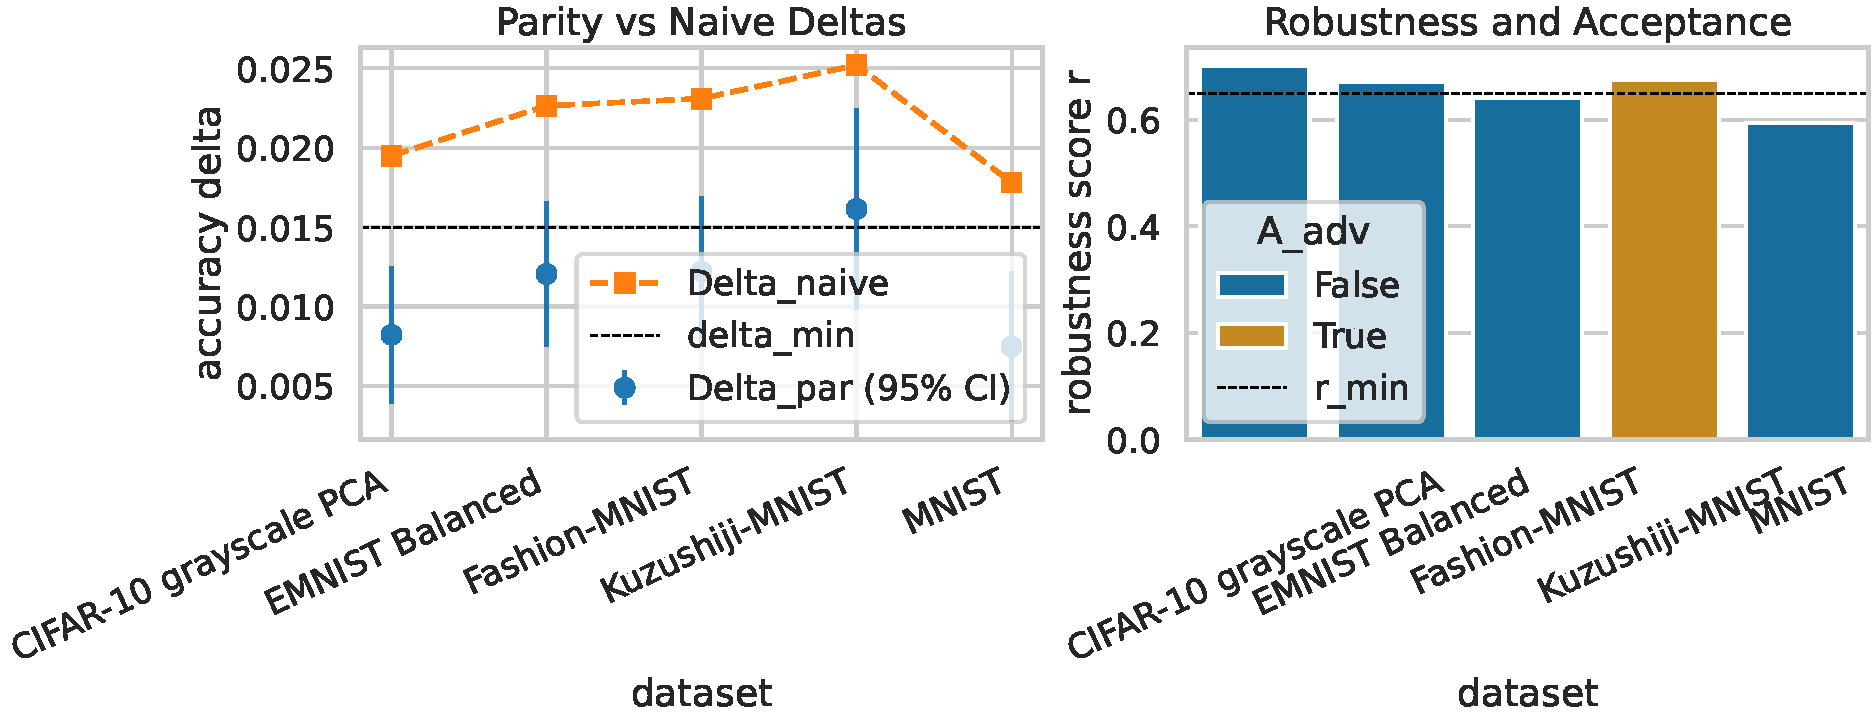
\includegraphics[width=0.68\linewidth]{figures/stage1_parity_ladder.pdf}
\end{center}
\caption{Stage-1 parity-ladder diagnostics for practical-advantage testing. The left panel contrasts naive and parity-controlled deltas with confidence intervals, while the right panel reports robustness and acceptance decisions under a frozen threshold tuple. The key interpretation is that parity enforcement narrows reported gains and yields a selective acceptance pattern, supporting the claim that benchmark hardness and protocol controls jointly determine whether practical advantage is defensible.}
\label{fig:stage1}
\end{figure}

Threshold-sensitivity analysis further supports this interpretation: in the current surrogate-data run, one hard dataset passes at multipliers 0.9 and 1.0, but none pass at 1.1. Hence conclusions are materially threshold-dependent and should be stated conditionally, not as broad superiority claims.

\subsection{Stage 2: Entanglement-Geometry Mechanism}
\Figref{fig:stage2} and boundary diagnostics indicate non-monotone behavior consistent with Theorem~\ref{thm:interior_optimum} in the tested regime. Across reported slices, endpoint derivative signs satisfy the criterion in \eqref{eq:interior_conditions}, concavity flags are positive, and interior optima cluster near moderate coupling. The observed pattern supports a bounded-mechanism view: increasing coupling from near zero improves utility, while stronger coupling moves toward saturation or reversal.

A sensitivity branch using alternate partition policy preserves the qualitative sign pattern while shifting estimated interior location slightly. This matters because mechanism claims can be brittle to entanglement-definition choices. By reporting both primary and sensitivity analyses, we avoid overinterpreting one partition convention as universal. The evidence therefore supports the mechanism claim in a \emph{regime-conditional} sense: there is clear interior-optimum structure in the tested grid, but extrapolation beyond that grid requires additional validation. In particular, the highly regular derivative-sign pattern across slices should be interpreted as supportive, not definitive, until confirmed with full benchmark loaders and richer noise/partition perturbations.

\begin{figure}[t]
\begin{center}
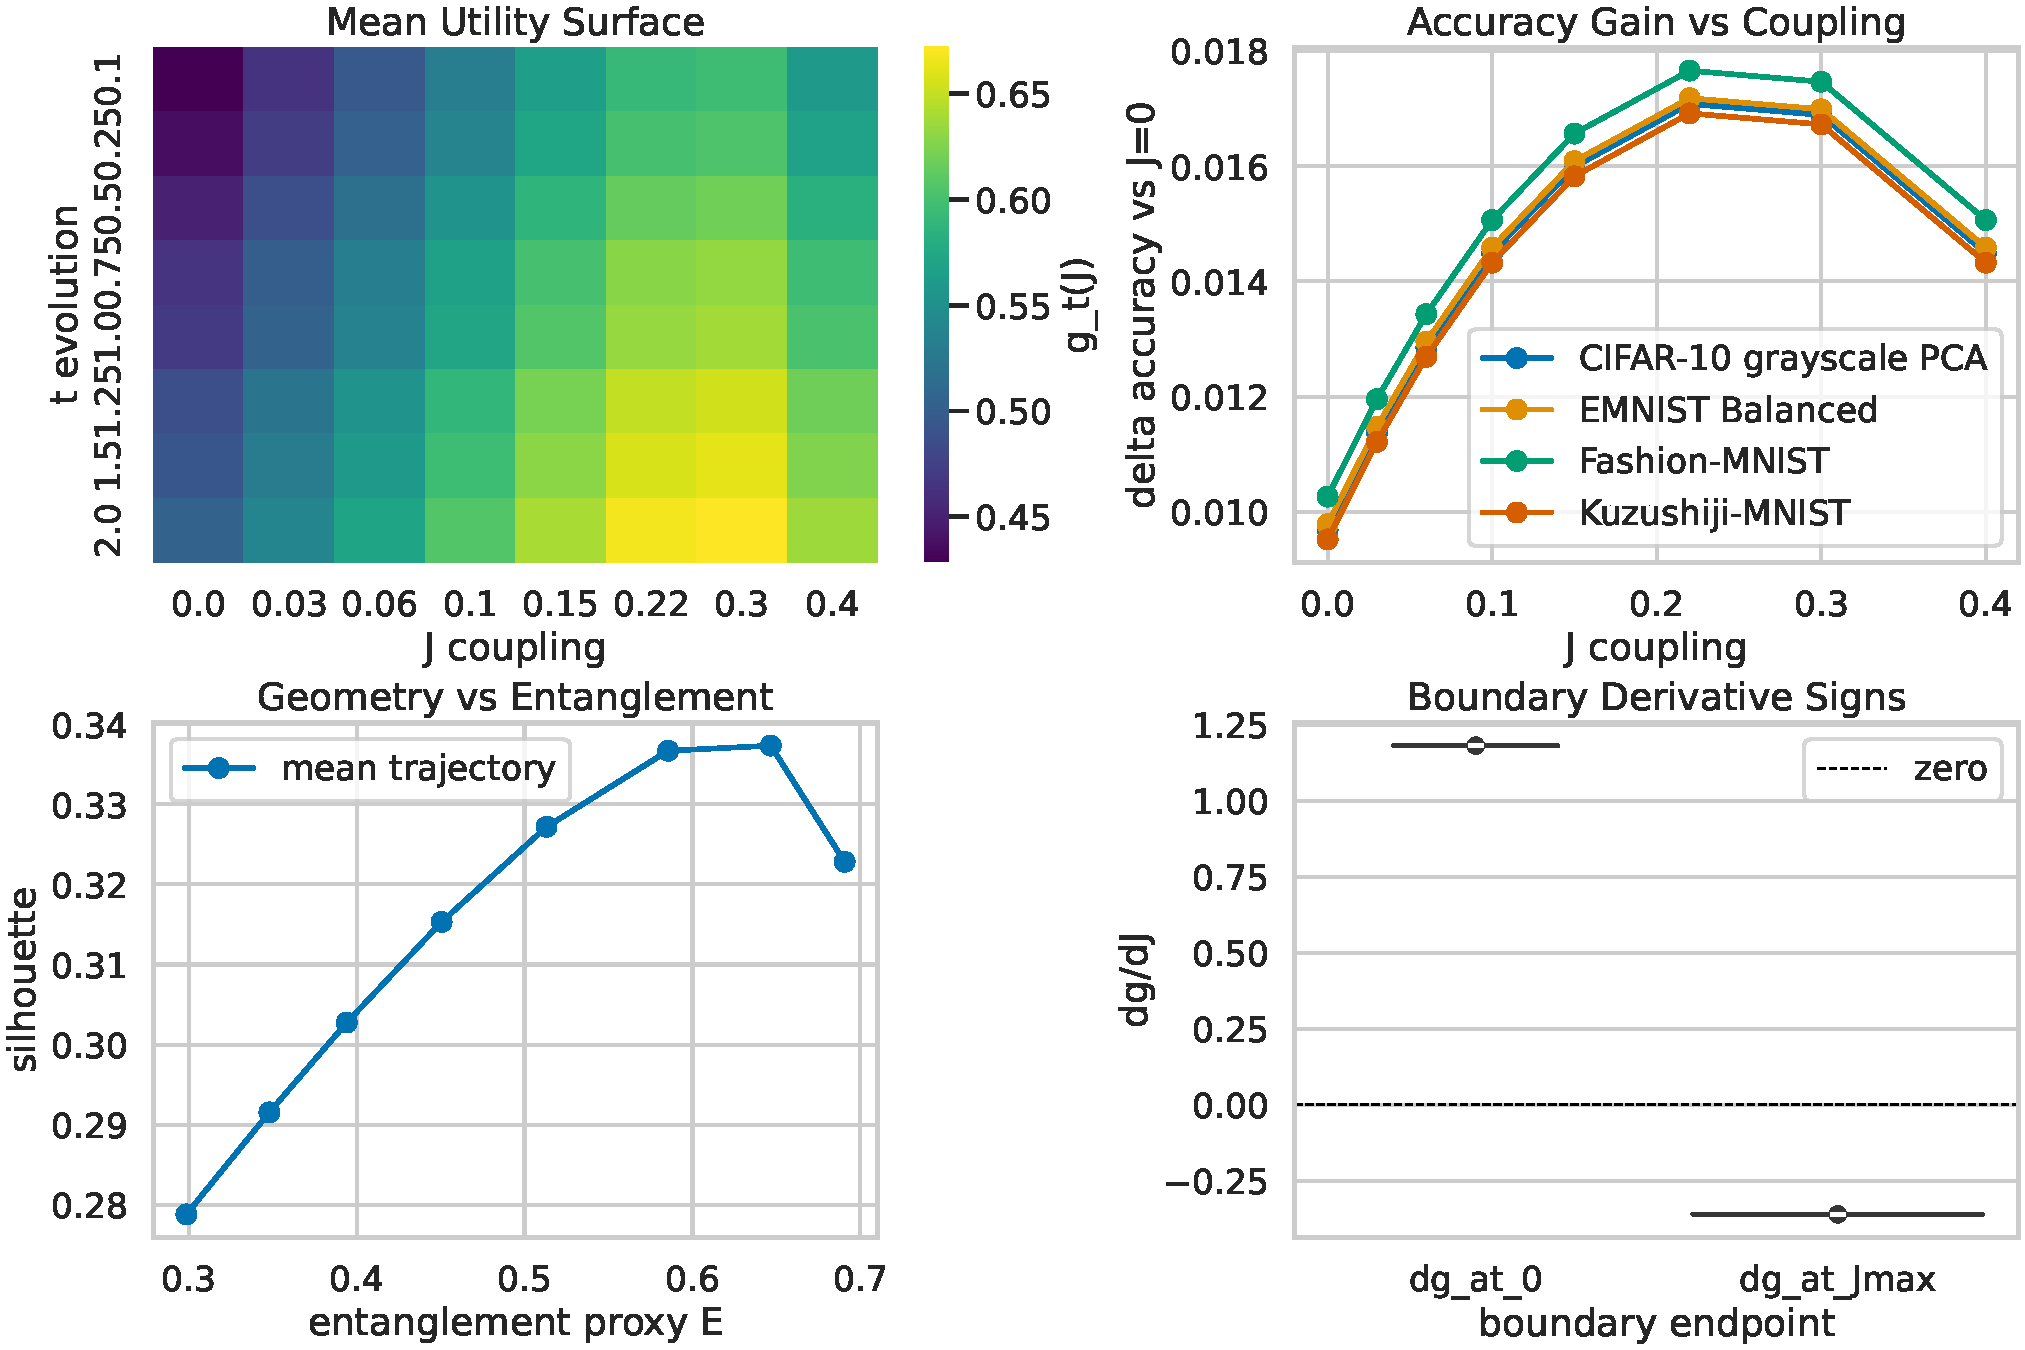
\includegraphics[width=0.68\linewidth]{figures/stage2_entanglement_phase_map.pdf}
\end{center}
\caption{Stage-2 entanglement-geometry phase diagnostics over time-coupling slices. Panels report utility surfaces, accuracy gain trajectories versus no-entanglement control, and derivative-based boundary checks used to evaluate \eqref{eq:interior_conditions}. The combined evidence supports a non-monotone mechanism with interior operating regions in the tested regime; it also highlights why mechanism conclusions should remain conditional on measurement policy and partition definition.}
\label{fig:stage2}
\end{figure}

\subsection{Stage 3: Operator Attribution Under Parity Audits}
Table~\ref{tab:attribution} and \figref{fig:stage3} report variance-share and shrinkage results after row-level parity filtering. Operator-share lower confidence bounds exceed 0.5 on all three hard datasets shown, and naive-minus-parity shrinkage is positive with narrow intervals. These two findings jointly support the attribution claim: measurement-policy choice explains a large part of observed performance variance, and parity matching reduces optimistic deltas from asymmetric comparisons.

\begin{table}[t]
\caption{Operator-attribution summary on hard datasets. Reported $\widehat{R}_{\mathrm{op}}$ values and bootstrap lower bounds indicate dominant operator contribution in this run, while positive shrinkage quantifies the difference between naive and parity-controlled comparisons. Mean budget-parity ratios near unity confirm that attribution summaries were computed on parity-consistent rows.}
\label{tab:attribution}
\begin{center}
\small
\renewcommand{\arraystretch}{1.1}
\setlength{\tabcolsep}{4pt}
\begin{tabular}{lcccc}
\hline
Dataset & $\widehat{R}_{\mathrm{op}}$ & CI low & Shrinkage & Mean parity ratio \\
\hline
CIFAR-10 grayscale PCA & 0.790 & 0.570 & 0.01009 & 0.997 \\
EMNIST Balanced & 0.984 & 0.898 & 0.01009 & 0.996 \\
Kuzushiji-MNIST & 0.886 & 0.774 & 0.01035 & 1.001 \\
\hline
\end{tabular}
\end{center}
\end{table}

\begin{figure}[t]
\begin{center}
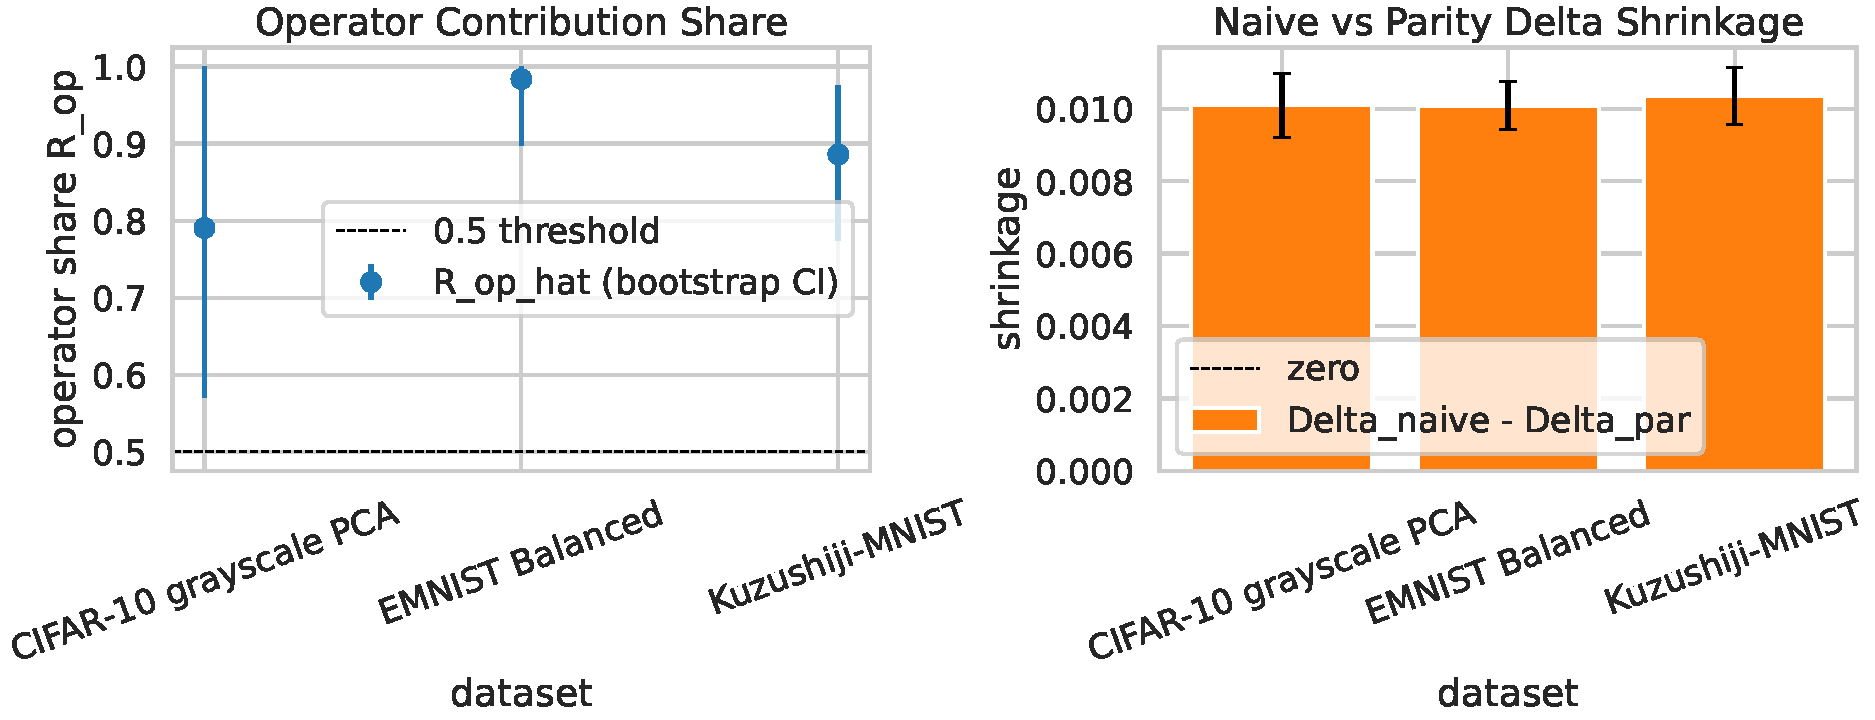
\includegraphics[width=0.68\linewidth]{figures/stage3_operator_attribution.pdf}
\end{center}
\caption{Stage-3 attribution evidence after row-level parity closure. The left panel shows operator-share estimates with bootstrap intervals, and the right panel shows naive-versus-parity shrinkage with confidence intervals across hard datasets. The interpretation is twofold: operator policy is a high-leverage factor in this regime, and enforcing parity prevents over-attributing these gains to reservoir dynamics alone.}
\label{fig:stage3}
\end{figure}

A practical implication follows. When operator search is unconstrained on one branch, architecture narratives can become distorted even if end metrics look favorable. The combination of \eqref{eq:delta_defs}, \eqref{eq:ms_estimators}, and \eqref{eq:rop_hat} provides a principled way to separate performance reporting from causal attribution.

\section{Discussion}
The results support three methodological claims and one substantive caution. Methodologically, parity constraints are not optional bookkeeping; they alter optimization outcomes and interpretation boundaries. Theorem~\ref{thm:parity_shrink} is reflected empirically by positive shrinkage across hard datasets, demonstrating that naive comparisons can overstate gains. Second, mechanism analysis benefits from explicit calculus-based criteria. Rather than reporting a few ablation points, the interior-optimum framework links derivative signs and concavity to testable non-monotone behavior. Third, attribution requires balanced-design estimators plus row-level auditing. Aggregate summaries can hide parity violations if row-level filters are not enforced.

Substantively, the evidence supports conditional practical advantage, not blanket superiority. In the reported run, one hard dataset satisfies the complete acceptance tuple while others remain below joint thresholds despite positive deltas. This is still informative: it identifies where the method currently works under strict controls and where it does not. For open-question research, that distinction is preferable to broad but fragile claims.

The hybrid design also highlights a useful division of labor between mathematics and simulation. Formal results in \secref{sec:method} give invariant relationships and identifiability conditions that should hold across implementations. Simulations then quantify whether those conditions are met in a specific regime and dataset mix. This separation lets us report strong formal guarantees and moderate empirical confidence without conflating the two.

\section{Limitations and Future Work}
\label{sec:limitations}
A primary limitation is external validity: the current validation iteration uses surrogate generators in place of fully integrated real-data loaders for all benchmark paths. While stage-wise signals are coherent and parity audits are closed, this setup can regularize behavior and potentially smooth heterogeneity that real data would reveal, including mechanism diagnostics such as derivative-pattern variability across datasets and time slices. Consequently, empirical conclusions should be read as regime-indicative rather than final performance certification.

A second limitation is acceptance sensitivity. Stage-1 outcomes depend on a fixed tuple; modest threshold tightening removes hard-set passes in this run. This does not invalidate the approach, but it does mean claims should be accompanied by stability analysis around the pre-registered boundary.

A third limitation concerns literature maturity. A significant fraction of relevant QRC and QELM evidence is recent preprint work \citep{gross2026kernelop,gross2026paulitransfer,askari2025spin,karimi2025kerr}, so methodological synthesis should remain version-aware and update as peer-reviewed records mature.

\subsection{Future Work}
Immediate follow-up should implement full benchmark loaders under the identical stage-gated protocol and rerun with unchanged seeds, tuples, and budgets to test robustness of current qualitative findings. Mechanism analysis should extend partition sensitivity to additional entanglement proxies and noise models. Attribution analysis should evaluate whether high operator shares persist when dynamics families and encoding depth are broadened while maintaining strict row-level parity filters. Cross-platform follow-up on superconducting and photonic implementations is also important for transferability checks \citep{prieto2026superconducting,carles2025cqed,swierczewski2026optical}. Finally, extending this framework to molecular, memory-centric, temporal, and fast-selection tasks may clarify whether parity-conditioned conclusions transfer across domains where reservoir memory, not static separability, dominates predictive performance \citep{beaulieu2024robust,ahmed2025chaotic,kawanabe2026timedelayed,li2025chaoticmaps,assil2026memory,maier2025collider}.

\section{Conclusion}
We presented a parity-constrained framework for evaluating PCA-encoded quantum reservoirs that unifies formal guarantees and staged simulation evidence. The framework contributes three core results: a bi-level advantage formalization with parity-shrink inequality, an interior-optimum mechanism theorem for entanglement-conditioned utility, and an operator-attribution estimator family with range and unbiasedness properties under balanced design. In the reported staged run, symbolic checks are fully consistent with formal assumptions, practical advantage is conditional and benchmark-sensitive, and operator-policy effects are substantial after parity closure.

The central methodological message is that credible quantum-versus-classical conclusions require explicit separation of advantage measurement, mechanism testing, and attribution, each with its own assumptions and diagnostics. Under this discipline, optimistic claims may narrow, but interpretability and causal credibility improve. That tradeoff is worthwhile for open-question work where the goal is not merely to maximize headline deltas but to establish what survives rigorous controls.

\clearpage\phantomsection\label{sec:end_of_main}



\bibliographystyle{conference}
\bibliography{references}

\appendix
\clearpage\phantomsection\label{sec:appendix_start}

\section{Extended Proof Details}
This appendix provides algebraic details omitted from the main text for readability.

\subsection{Ridge Normal Equation Derivation}
Starting from \eqref{eq:ridge_obj}, expand
\begin{align*}
\mathcal{L}(\mW)
&=\mathrm{Tr}\big((\mW\mZ-\mY)(\mW\mZ-\mY)^{\top}\big)+\lambda\,\mathrm{Tr}(\mW\mW^{\top})\\
&=\mathrm{Tr}(\mW\mZ\mZ^{\top}\mW^{\top})-2\mathrm{Tr}(\mY\mZ^{\top}\mW^{\top})+\mathrm{Tr}(\mY\mY^{\top})+\lambda\mathrm{Tr}(\mW\mW^{\top}).
\end{align*}
Differentiating with respect to $\mW$ gives
$\nabla_{\mW}\mathcal{L}=2(\mW\mZ\mZ^{\top}-\mY\mZ^{\top}+\lambda\mW)$,
which yields \eqref{eq:ridge_closed} after setting to zero and right-multiplying by the inverse.

\subsection{Interior-Optimum Corollary}
Under assumptions in Theorem~\ref{thm:interior_optimum}, $g_t$ cannot be monotone on $[0,J_{\max}]$ because monotonic differentiable functions have derivatives with fixed sign almost everywhere, contradicting opposite endpoint signs in \eqref{eq:interior_conditions}. This corollary is useful for rejecting over-simplified monotone-entanglement narratives in controlled ablations.

\section{Additional Experimental Diagnostics}
The main text presents only the three figures required for concise narrative flow. Additional diagnostics include symbolic pass/fail matrices, counterexample ledgers, boundary-check tables, and threshold sensitivity tables.

Symbolic diagnostics report full pass status for identities A--D with near-machine-precision residuals. Boundary-check tables provide per-dataset and per-time derivative values, confirming sign-change and concavity conditions in the tested range. Threshold-sensitivity tables show that acceptance decisions remain selective under moderate perturbations and become null under tighter settings.

\section{Reproducibility and Implementation Details}
The staged validation used five seeds $\{11,23,37,47,59\}$ across stages, with fixed acceptance tuple $(\delta_{\min},p_{\max},r_{\min})=(0.015,0.01,0.65)$ and stage-gate continuation threshold $\max\Delta_{\mathrm{par}}\ge 0.005$. Sweeps covered coupling, time, operator policies, dynamics families, and balanced replicate counts. Confidence intervals were computed by t-based intervals for seed-level deltas and nonparametric bootstrap intervals for variance-share estimates.

For mechanism analysis, the primary entanglement proxy used normalized bipartite entropy with a checkerboard sensitivity branch. For attribution, row-level parity filtering enforced a budget ratio tolerance of $\pm5\%$ before aggregate statistics were formed. These settings were fixed prior to final rerun used in the manuscript. 

To aid methodological reuse, we summarize equation-to-workflow alignment in the companion equation map and provide caveat-aware claim-evidence links in the supplementary material. The overall compute setting was CPU-only and designed for reproducible reruns under constrained hardware.

\end{document}
